\documentclass[11pt]{article}
\usepackage{geometry, titlesec}
\usepackage[parfill]{parskip}
\usepackage[italicdiff]{physics}
\usepackage{amsfonts, amsthm}
\usepackage[cm]{fullpage}
\usepackage{fancyhdr}
\usepackage{enumitem}
\usepackage{xcolor, soul}
\usepackage{graphicx}
\usepackage[export]{adjustbox}
\usepackage{siunitx}
%\allowdisplaybreaks

\renewcommand{\thesubsection}{\thesection.\alph{subsection}}
\setenumerate[1]{label={(\alph*)}}

\makeatletter
\renewcommand*\env@cases[1][1.2]{%
  \let\@ifnextchar\new@ifnextchar
  \left\lbrace
  \def\arraystretch{#1}%
  \array{@{}l@{\quad}l@{}}%
}
\makeatother
 
\renewcommand{\footrulewidth}{.2pt}
%\setlist[enumerate]{leftmargin=*}
\pagestyle{fancy}
\fancyhf{}
\lhead{Physics 132-B}
\chead{\textbf{Discussion 8 Problems}}
\rhead{A--De Discussion}
\setlength{\headheight}{11pt}
\setlength{\headsep}{11pt}
\setlength{\footskip}{24pt}
\lfoot{\today}
\rfoot{\thepage}

\titleformat{\subsection}[runin]{\normalfont\large\bfseries}{\thesubsection}{1em}{}
\newcommand{\refeq}[1]{(\ref{#1})}

\newcommand{\beq}{\begin{equation*}}
\newcommand{\eeq}{\end{equation*}}

\newcommand{\beqn}{\begin{equation}}
\newcommand{\eeqn}{\end{equation}}

\newcommand{\blg}{\begin{align*}}
\newcommand{\elg}{\end{align*}}


\newenvironment{statement}
{
%    \color{gray}
    \ignorespaces
}
{
%    \smallskip
}

\newenvironment{problem}
{
%    \color{darkgray}
    \ignorespaces
}

\newenvironment{solution}
{
    \paragraph{Solution.}
    \ignorespaces
}
{
    \bigskip
}

\newcommand{\qimplies}{\quad \implies \quad}
\renewcommand{\medskip}{\vspace{8pt}}


\begin{document}
	


\newcommand{\vB}{\vb{B}}

\paragraph{Question 29.1}
\begin{problem}
	A sheet of copper is placed between the poles of an electromagnet with the magnetic field perpendicular to the sheet.  When the sheet is pulled out, a considerable force is required, and the force required increases with speed.  Explain.  Is a force required also when the sheet is inserted between the poles?  Explain.
\end{problem}

\vfill

\paragraph{Question 29.3}
\begin{problem}
	Two circular loops lie side by side in the same plane.  One is connected to a source that supplies an increasing current; the other is a simple closed ring.  Is the induced current in the ring in the same direction as the current in the loop connected to the source, or opposite?  What if the current in the first loop is decreasing?  Explain.
\end{problem}

\vfill

\paragraph{Question 29.13}
\begin{problem}
	A metal ring is oriented with the plane of its area perpendicular to a spatially uniform magnetic field that increases at a steady rate.  If the radius of the ring is doubled,
	\begin{enumerate}
		\item by what factor does the emf induced in the ring change, and
		\item by what factor does the electric field induced in the ring change?
	\end{enumerate}
\end{problem}

\vfill

\clearpage


\newcommand{\PhiB}{\Phi_B}

\begin{minipage}[l]{0.65\textwidth}
\paragraph{Problem 29.7}
\begin{problem}
	The current in the long, straight wire shown in \textbf{Fig.~E29.7} is upward and is increasing steadily at a rate $\dv*{i}{t}$. \medskip
	\begin{enumerate}
		\item At an instant when the current is $i$, what are the magnitude and direction of the field $\vB$ at a distance $r$ to the right of the wire?  (Use Ampere's law to find the magnitude.) \medskip
		\item What is the flux $\dd{\PhiB}$ through the narrow, shaded strip? \medskip
		\item What is the total flux through the loop? \medskip
		\item What is the induced emf in the loop? \medskip
		\item Evaluate the numerical value of the induced emf if $a = \SI{12.0}{\cm}$, $b = \SI{36.0}{\cm}$, $L = \SI{24.0}{\cm}$, and $\dv*{i}{t} = \SI{9.60}{\ampere\per\second}$.
	\end{enumerate}
\end{problem}
\end{minipage}%
\hspace{0.05\textwidth}%
\begin{minipage}[r]{0.30\textwidth}
\center 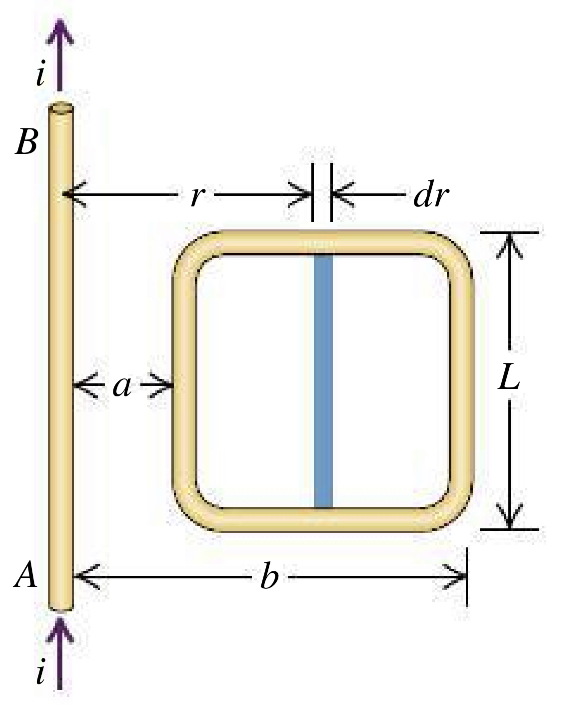
\includegraphics[width=\textwidth]{P29-7.jpeg}
\center \textbf{Figure E29.7}
\end{minipage}

\vfill 

\end{document}